\documentclass[journal=jpcbfk]{achemso}

\usepackage[version=3]{mhchem}
\usepackage[T1]{fontenc}
\newcommand*\mycommand[1]{\texttt{\emph{#1}}}
\newcommand{\todo}[1]{\textcolor{red}{#1}}

\usepackage{upgreek}				
\usepackage{xcolor}
\usepackage{booktabs}
\usepackage{multirow}
\usepackage{lmodern}
\usepackage{microtype}


\author{Josef Melcr}
\author{Hector Martinez-Seara}
\affiliation{Institute of Organic Chemistry and Biochemistry,
Academy of Sciences of the Czech Republic, 
Prague 6, Czech Republic}
\author{Ji{\v r}{\' i} Kolafa}
\affiliation{Department of Physical Chemistry, Institute of Chemical Technology, Prague 6, Czech Republic}
\author{Pavel Jungwirth}
\affiliation{Institute of Organic Chemistry and Biochemistry,
Academy of Sciences of the Czech Republic, 
Prague 6, Czech Republic}
\alsoaffiliation{Department of Physics, Tampere University of Technology, P.O. Box 692, FI-33101
Tampere, Finland}

\author{O. H. Samuli Ollila}
\email{samuli.ollila@helsinki.fi}
%\homepage[]{Your web page}
\affiliation{Institute of Organic Chemistry and Biochemistry,
Academy of Sciences of the Czech Republic, 
Prague 6, Czech Republic}
\alsoaffiliation{Institute of Biotechnology, University of Helsinki}




\SectionNumbersOn

\renewcommand{\thetable}{S\arabic{table}}%
\renewcommand{\thefigure}{S\arabic{figure}}%
\renewcommand{\thesection}{S\arabic{section}}%
\renewcommand{\thepage}{S\arabic{page}}%

\title{Supporting Information:\\Accurate binding of sodium and calcium to phospholipid bilayers by effective inclusion of electronic polarization}

\begin{document}

\newpage
%\tableofcontents

\section{Simulation details}

\begin{table}[!h]
  \caption{Simulation parameters}
  \label{tbl:mdpar}
  \begin{tabular}{ll}
    simulation property & parameter   \\
    \hline
    time-step           & 2~fs         \\
    equilibration time  & 100~ns  \\
    total simulation time     & 300~ns  \\
    temperature         & 313~K       \\
    thermostat          & v-rescale  \cite{bussi07}   \\
    barostat            & Parrinello-Rahman, semi-isotropic \cite{parrinello81} \\
    long-range electrostatics & PME  \cite{darden93}  \\
    cut-off scheme      & Verlet \cite{Pall13}      \\
    Coulomb and VdW cut-off & 1.0~nm \\
    constraints         & LINCS, only hydrogen atoms \cite{hess97} \\
    constraints for water & SETTLE  \cite{miyamoto92} \\
    \hline
  \end{tabular}
\end{table}

OpenMM simulations were run with 4~fs time step using 4 times heavier hydrogen atoms (mass subtracted from neighbouring atoms). 

\newpage
\section{Area per molecule and calcium binding with different water models}

\begin{table}[!h]
  \caption{Area per lipid (APL) from different models of POPC with no ions\label{tab:apls_si} }
  \begin{tabular}{l|c c}
    model          & APL (\AA$^2$)   & Temperature [K] \\
    \hline
    Lipid14                   & 65.1$\pm$ 0.6  &  300 \\
    Lipid14 \cite{dickson14}  & 65.6$\pm$ 0.5  &  303 \\
    \hline
    ECC-POPC &        &  \\
    ~ SPC/E          & 63.2$\pm$ 0.6   &  300       \\
    ~ SPC/E          & 65.1$\pm$ 0.6   &  313       \\
    ~ OPC3           & 62.2$\pm$ 0.6   &  300       \\
    ~ OPC3           & 64.2$\pm$ 0.6   &  313       \\
    ~ OPC            & 64.4$\pm$ 0.6   &  313       \\
    ~ TIP4p/2005     & 66.8$\pm$ 0.6   &  313       \\
    ~ TIP3p          & 66.2$\pm$ 0.6   &  313       \\
    ~ TIP3p-FB       & 64.8$\pm$ 0.6   &  313       \\
    ~ TIP4p-FB       & 65.6$\pm$ 0.6   &  313       \\
    \hline
    experiment \cite{kucerka11}  & 62.7$\pm$ 1.3  &  293    \\
                                 & 64.3$\pm$ 1.3  &  303    \\
                                 & 67.3$\pm$ 1.3  &  323    \\
                                 & 68.1$\pm$ 1.4  &  333    \\
    %experiment POPE  & 56.6 &  303    \\
    \hline
  \end{tabular} \\
\end{table}


\begin{figure}[!hp]
  \centering
  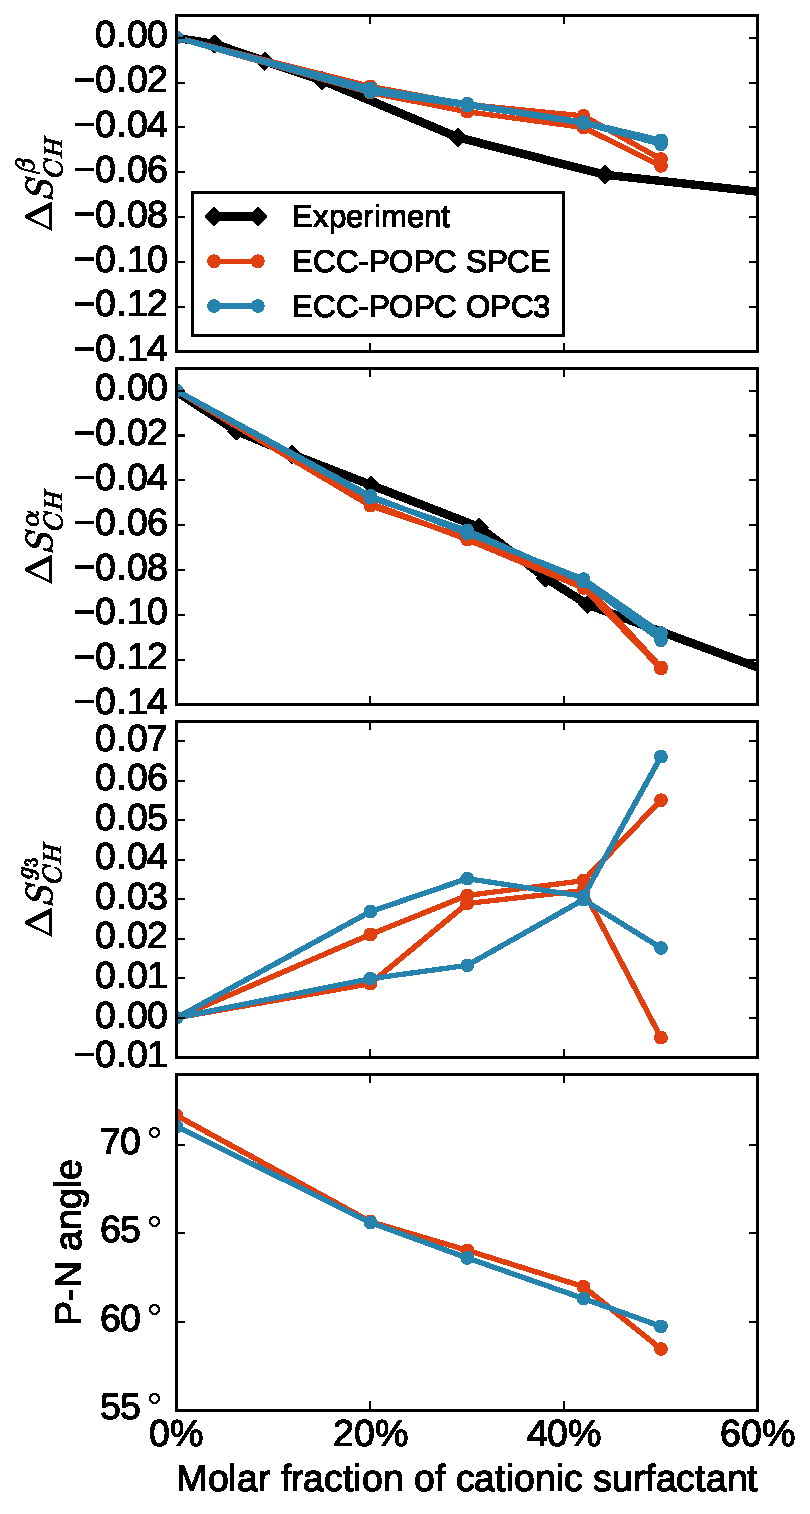
\includegraphics[width=8.0cm]{../Fig/ipython_nb/PN_angle_OrdPars-A-B-g3_L14-ECCL17_q80_sig89_surf_waterModels_compar.pdf}
  \caption{\label{fig:ordPars_waterModels_surf}
    Changes of head group and glycerol carbon $g_3$ order parameters, and P-N vector orientation of POPC bilayer
    as a function of a molar fraction of the cationic surfactant dihexadecyldimethylammonium in a POPC bilayer
    from simulations with different water models (OPC3~\cite{Izadi16}, SPC/E~\cite{Berendsen1987})
    and experiments \cite{scherer89} at 313 K.
  }
\end{figure}

\begin{figure}[!hp]
  \centering
  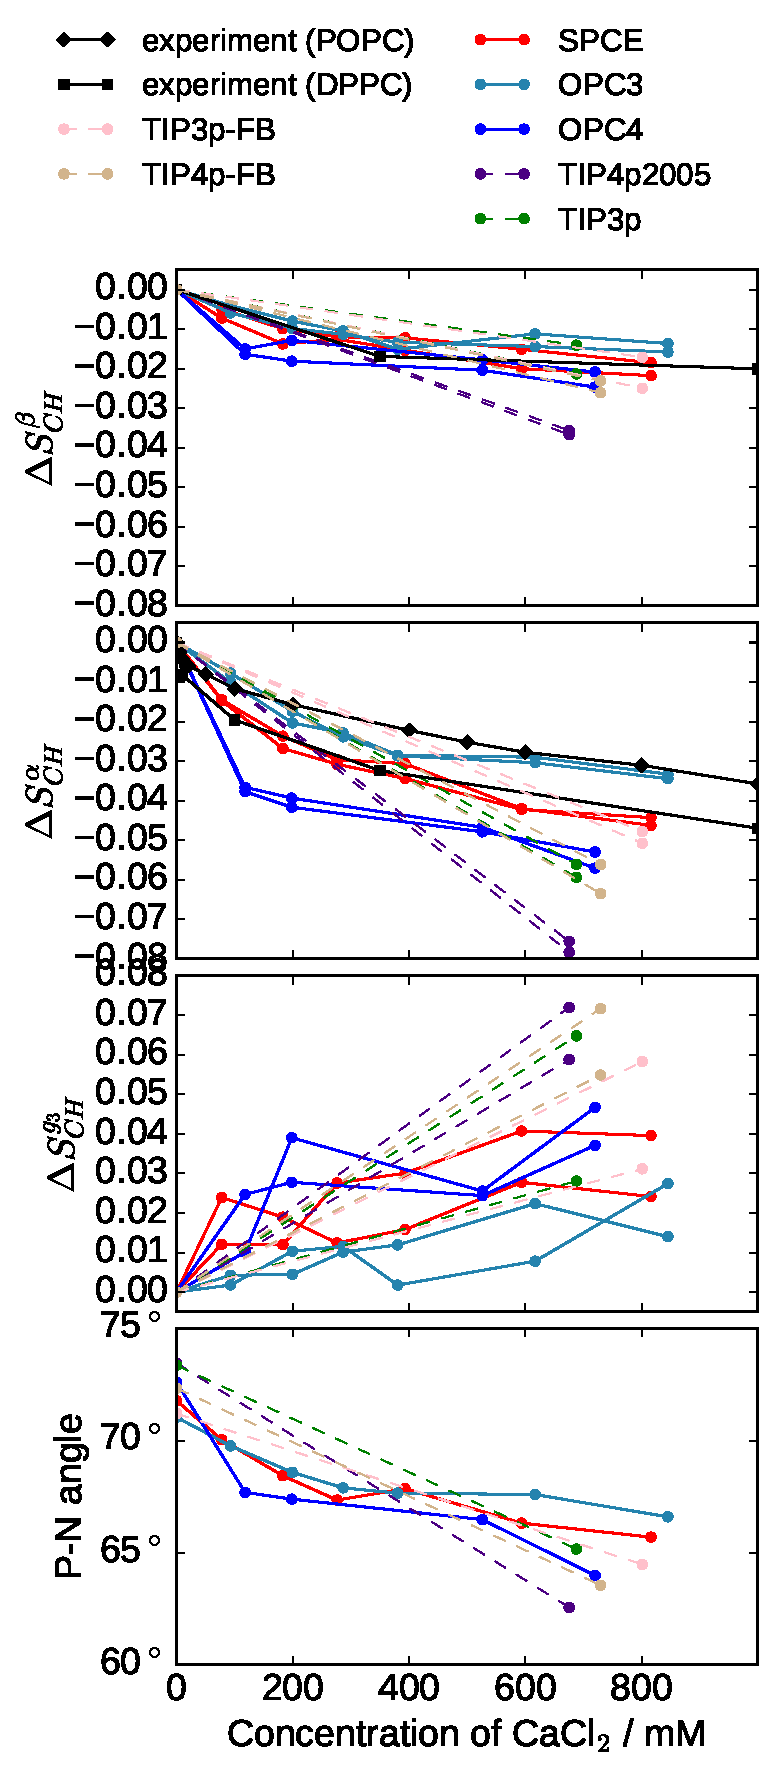
\includegraphics[width=8.0cm]{../Fig/ipython_nb/PN_angle_OrdPars-A-B-g3_L14-ECCL17_q80_sig89_CaCl_waterModels.pdf}
  \caption{\label{fig:ordPars_waterModels}
    Changes of head group and glycerol carbon $g_3$ order parameters, and P-N vector orientation of POPC bilayer
    as a function of CaCl$_2$ concentrations in bulk ($C_{ion}$) from ECC-POPC simulations at 313K with different
    water models (SPC/E~\cite{Berendsen1987}, OPC \cite{Izadi14}, OPC3~\cite{Izadi16}, TIP3P~\cite{jorgensen83}, TIP3p-FB and TIP4p-FB~\cite{Wang2014}, and TIP4p/2005 \cite{Abascal2005})
    together with experimental data (DPPC (323~K) \cite{akutsu81} and POPC (313~K) \cite{altenbach84}). 
    Ion concentrations ($C_{ion}$) are calculated from the cation number density $C_{np}$
    at the farthest point from the lipid bilayer in the aqueous phase as [ion]=$C_{np}/0.602$.
  }
\end{figure}


\newpage
\section{Sodium binding to POPC with the glycerol carbon $g_3$ order parameters and the head group orientation}

\begin{figure}[!h]
  \centering
  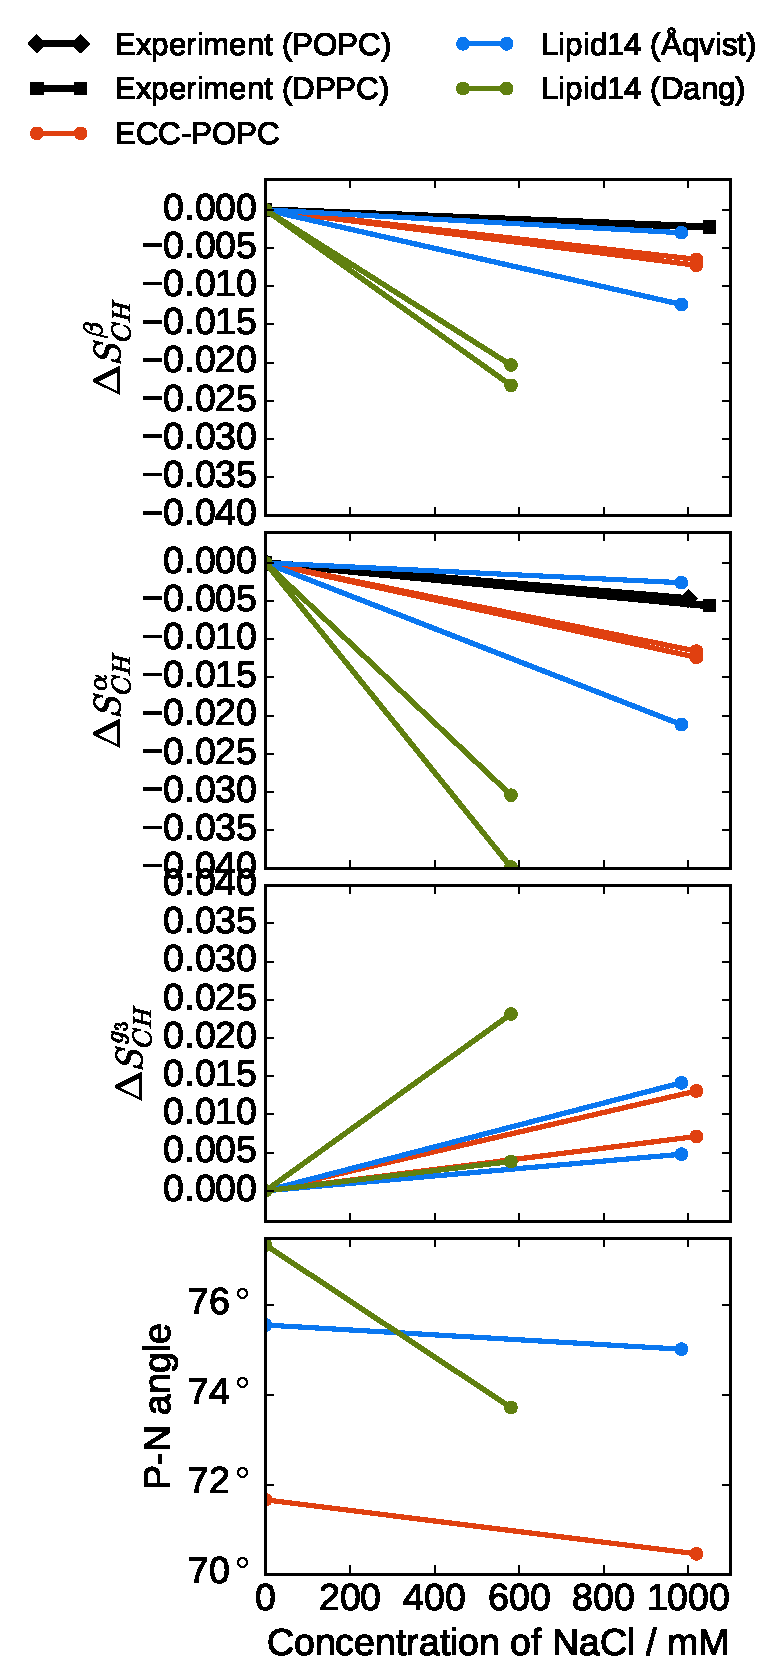
\includegraphics[width=8.0cm]{../Fig/ipython_nb/PN_angle_OrdPars-A-B-g3_L14-ECCL17_q80_sig89_NaCl.pdf}
  \caption{\label{fig:delta_ordPar_NaCl_si}
    Changes of head group and glycerol carbon $g_3$ order parameters, and the P-N vector orientation of POPC bilayer
    as a function of NaCl concentrations in bulk ($C_{ion}$)
    from simulations with different force fields at 313~K together with experimental
    data (DPPC (323~K)~\cite{akutsu81} and POPC (313~K)~\cite{altenbach84}). 
%    Ion concentrations in bulk water are shown in x-axis. 
%    Values from simulations are calculated from the of cation number density $C_{np}$
%    from the region at the simulatin box edge with the constant ion concentration as [ion]=$C_{np}/0.602$.
    Simulation data with Lipid14 and \AA{}qvist ion parameters at 293~K is taken directly
    from Refs.~\citenum{catte16,lipid14POPC0mMNaClfiles,lipid14POPC1000mMNaClfiles}.
  }
\end{figure}


\section{Ternary complex model in simulations}
The NMR data about PC headgroup order parameters
and atomic absorption spectroscopy data were previously
best explained using a ternary complex binding model~\cite{altenbach84}.
In this model, one calcium is assumed to form
complexes with two lipids, i.e. with the binding stoichiometry of~1~\ce{Ca^{2+}}:2~POPC.
The model predicts a linear relationship between quantities 
$C_b$ and $\sqrt{C_b/C_I}$, where $C_b$ is the
mole fraction of bound \ce{Ca^{2+}} per POPC
and $C_I$ is the concentration of free cations at the plane of ion binding~\cite{altenbach84}.
Experimentally detemined $C_b$ %was obtained from an extrapolation of linear relation 
from NMR measurements and atomic absorption spectroscopy %for low concetrations of \ce{CaCl2}.
%Such an extrapolation is valid as long as the mode of \ce{Ca^{2+}} binding 
%remains constant throughout the extrapolation range. 
together with $C_I$ calculated from the Poisson-Boltzmann equation
gave a good agreement with the predictions of the
ternary complex model~\cite{altenbach84}.

To compare ECC-POPC simulations to the ternary complex model,
%An atomistic simulation, on the other hand, provides these quantities directly without severe assumptions;
we calculated $C_b$ from simulations (as defined in the main text),
and $C_I$ from the minimum CaCl$_2$ concentration at membrane-water interface,
%the shallow depression separating the bulk water phase 
locating around 2.6\,nm from the membrane center in
the density profiles in Fig.~5 in the main text. 

The results from simulations are shown in Fig.~\ref{fig:cacl-bind}
together with the line fitted to experimental data by Altenbach and Seelig~\cite{altenbach84}.
Both results are in agreement with the prediction of the ternary complex model.
The small discrepancy between the results from experiments and simulations probably
arise from difference in the evaluation of the concentrations and
inaccuracy of Poisson-Boltzmann theory for divalent cations like \ce{Ca^{2+}}~\cite{Andelman1995}. 
In conclusion, the results suggest that the almost equal probabilities for
\ce{Ca^{2+}} to form complexes with one to three lipids detailed in the main text is in line with an averaged interpretation of the experimental observations which supported the ternary complex model.
\newpage
\begin{figure}[!h]
  \centering
  \includegraphics[height=9.0cm,angle=-90]{../Fig/bound-CAs_conc-eccl17.eps}
  \caption{\label{fig:cacl-bind}
    Fits of experimental~\cite{altenbach84} and ECC-POPC simulation data to
    the prediction of the ternary complex model.
    %{\color{red} Joe, please change the axes labels to correspond the notation in the text, i.e. $C_b$ and $C_I$,
    %and write in the title of simulation fit (red dashed line) that it is the fit to simulation.}
    %Ternary complex binding model of \ce{Ca^{2+}} to a POPC membrane 
    %that assumes the stoichiometry of 2~POPC:1~\ce{Ca^{2+}} (details in reference~\citenum{altenbach84}) 
    %provides a good fit to experimental measurements~\cite{altenbach84}
    %and it also provides a good fit to our simulation data. 
    %This supports our statement that the success of the ternary complex model in the experiments
    %can be understood with the atomistic detail of our simulations as an average 
    %stoichiometry of otherwise almost evenly distributed clusters of one cation with 1,2 or 3 lipids (Fig.~\ref{fig:cacl_complexes}). 
    %Note that the units in the reference~\citenum{altenbach84} are different from the units presented here,
    %and, hence, the observed slope of the linear relationship is slightly different.
    }
\end{figure}

\newpage
\section{Histograms of residence times}

\begin{figure}[!h]
  \centering
  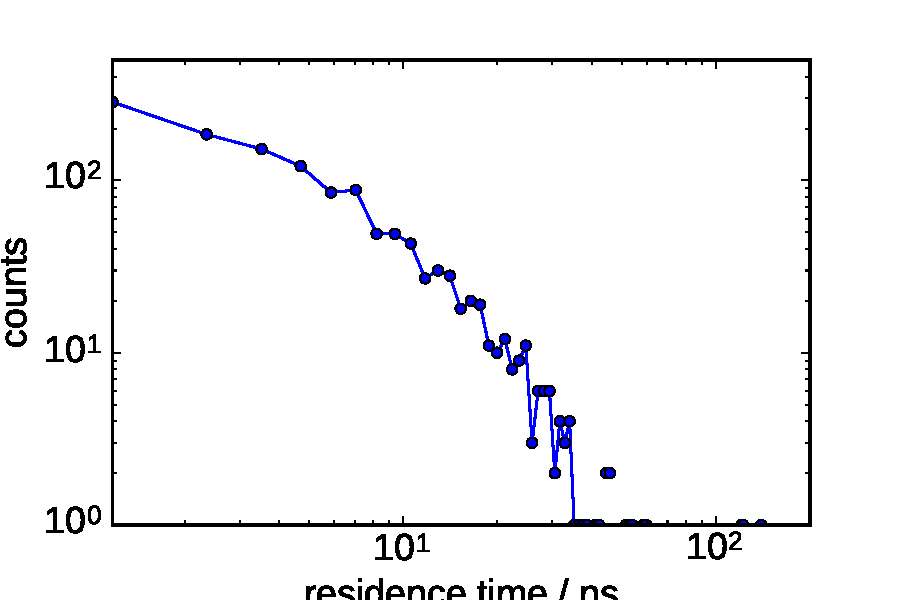
\includegraphics[width=8.0cm]{../Fig/ipython_nb/histogram_bound_times_ECC-lipids_346mM_CaCl.pdf} \\
  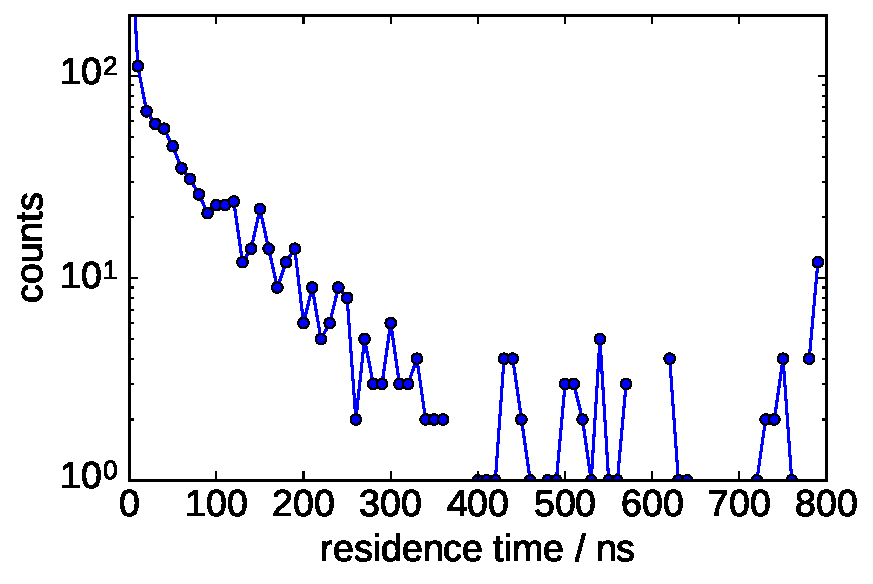
\includegraphics[width=8.0cm]{../Fig/ipython_nb/histogram_bound_times_Charmm36_450mM_CaCl_Matti.pdf}
  \caption{\label{fig:hist_residence_times}
   Histograms of residence times of \ce{Ca^{2+}} in a POPC bilayer
   from ECC-POPC (top) and CHARMM36 (bottom) simulations with ECC-ions.
   Both simulations had the same concentration of \ce{CaCl_2} respect to water ($C_{ion}'$= 450~mM).
   CHARMM36 simulation was directly taken from Refs.~\citenum{javanainen17,zenodo.259376}.
   Scales of x-axes represent the lengths of the simulations used for analysis.
   In ECC-POPC simulation, 90\% of the residence times are
   shorter than $60\,\mathrm{ns}$, % exactly $53\,\mathrm{ns}$                                                                          
   with the longest observed residence time being $141\,\mathrm{ns}$,
   which is well below the total length of the simulation (200~ns).
   This is, however not the case in CHARMM36 simulation,
   where residence times of several calcium cations are    
   apparently limited by the length of the simulation.
   %With such a simulation, which is relatively short for the employed model,
   %we can merely estimate an upper bound that
   %only
   Less than 60\% of the residence times are
   %is formed by cations interacting with the phospholipid membrane
   shorter than the half of the simulation length~(400~ns)
   in CHARMM36 simulation.
  }
\end{figure}

\newpage
\section{Comparison between Gromacs and openMM}

\begin{figure}[!h]
  \centering
  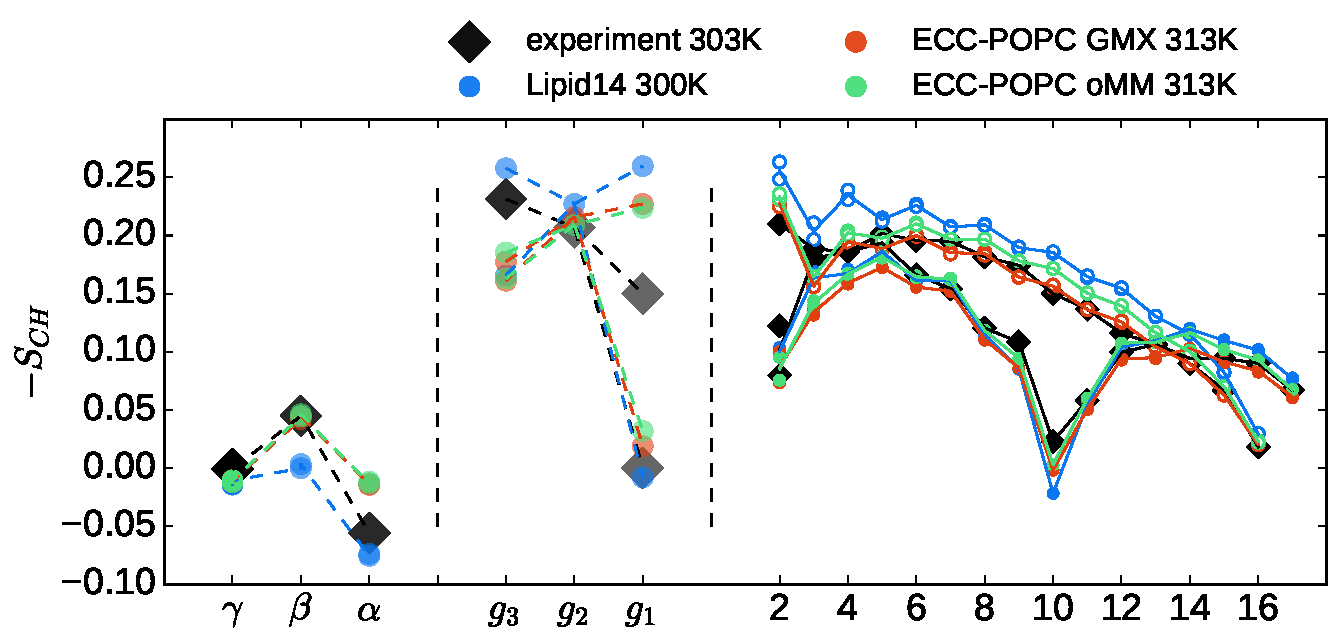
\includegraphics[width=16.0cm]{../Fig/ipython_nb/Order-parameters_exp-L14-ECCL17_q80_sig89_GMX-oMM_compar.pdf}
  \caption{\label{fig:ordPars_actual_GMX_oMM_compar}
    Order parameters of POPC head group, glycerol backbone and acyl chains 
    from Lipid14 \cite{dickson14} and ECC-POPC simulations ran
    with GROMACS~5.1.4 \cite{Abraham15} and openMM~7 \cite{openmm7} 
    together with experiments~\cite{ferreira13}.
    The size of the markers for the head group order parameters correspond to
    the error estimate $\pm 0.02$ for experiments \cite{botan15,ollila16},
    while the error estimate for simulations is $\pm 0.005$.
    The size of the points for acyl chains are decreased by a factor of 3 to improve the clarity of the plot.
  }
\end{figure}

\begin{figure}[!p]
  \centering
  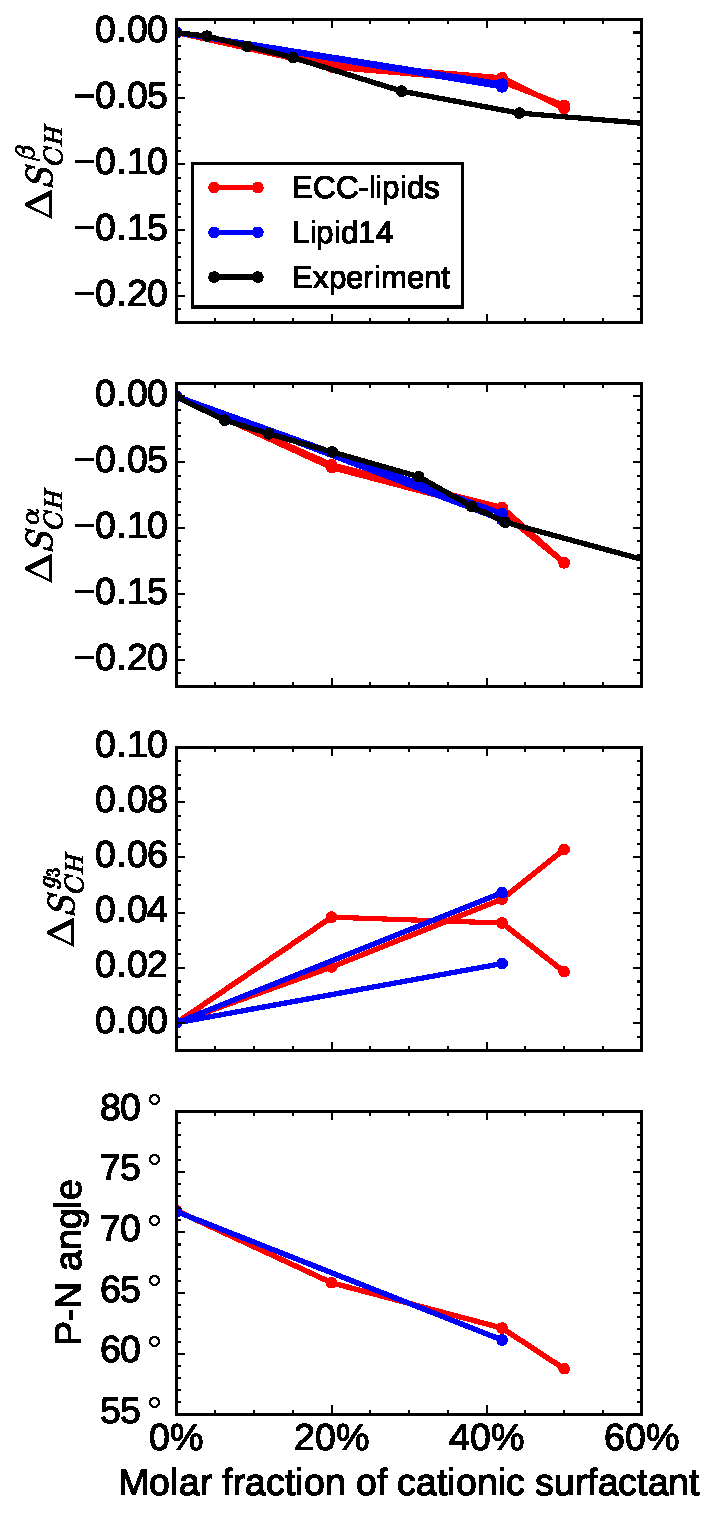
\includegraphics[width=8.0cm]{../Fig/ipython_nb/PN_angle_OrdPars-A-B-g3_L14-ECCL17_q80_sig89_surf_GMX-oMM_compar.pdf}
  \caption{\label{fig:ordPars_surf_GMX_oMM_compar}
    Changes of headgroup and glycerol carbon $g_3$ order parameters, and P-N vector orientation as a function of
    a molar fraction of the cationic surfactant dihexadecyldimethylammonium in a POPC bilayer
    from simulations with the ECC-POPC model
    simulated with GROMACS~5.1.4 \cite{Abraham15} and openMM~7 \cite{openmm7} 
    compared with the experimental values from \cite{scherer89}.
    The size of the markers for the head group order parameters correspond to
    the error estimate $\pm 0.02$ for experiments \cite{botan15,ollila16},
    while the error estimate for simulations is $\pm 0.005$.
  }
\end{figure}

\begin{figure}[!p]
  \centering
  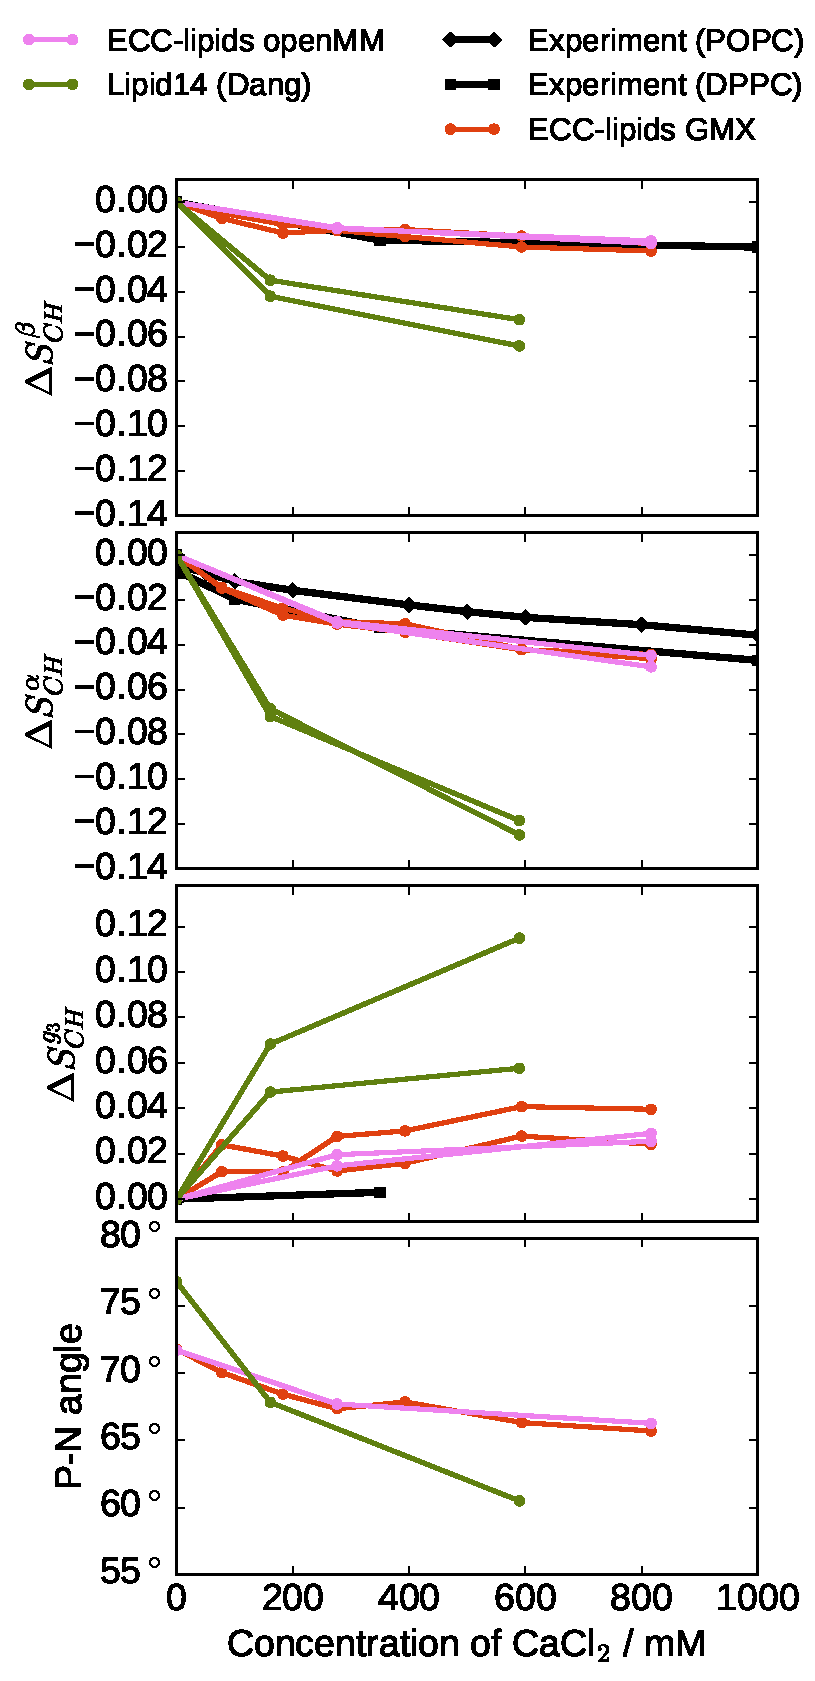
\includegraphics[width=8.0cm]{../Fig/ipython_nb/PN_angle_OrdPars-A-B-g3_L14-ECCL17_q80_sig89_CaCl_GMX-oMM_compar.pdf}
  \caption{\label{fig:ordPars_cacl_GMX_oMM_compar}
    Changes of the head group and glycerol carbon $g_3$ order parameters, and P-N vector orientation of a POPC bilayer 
    as a function of the CaCl$_2$ concentration in bulk ($C_{ion}$)
    from Lipid14 \cite{dickson14} and ECC-POPC simulations ran
    with GROMACS~5.1.4 \cite{Abraham15} and openMM~7 \cite{openmm7} at 313~K
    together with experiments (DPPC (323\,K) \cite{akutsu81} and POPC (313\,K) \cite{altenbach84}). 
    %Ion concentrations in bulk water are shown in x-axis. 
    Bulk concentrations from simulations are calculated 
    from the farthest point from the lipid bilayer in the aqueous phase
    with an error estimate of 10\,mM.
  }
\end{figure}



\newpage
\bibliography{refs.bib}

\end{document}
